\documentclass[a4paper]{article}
\title{TP1 : Ghostbusters \protect\\ Programmation temps-réel}
\author{Groupe 2 \\ Orphée Antoniadis \hspace{0.5cm} Raed Abdennadher \hspace{0.5cm} Steven Liatti}
\usepackage[francais]{babel}
\usepackage{fontspec}
\usepackage{amsmath}
\usepackage{amsfonts}
\usepackage{enumitem}
\usepackage{minted}
\usemintedstyle{colorful}
\setlength{\parindent}{0pt}
\usepackage[left=2cm,top=2cm,right=2cm,bottom=2cm]{geometry}
\usepackage{caption}

\begin{document}
\maketitle

\section{Introduction}
Le but de ce travail était de réaliser un jeu qui est un mélange entre deux
anciens jeux vidéo : le Pacman et le Casse-brique. L'objectif était d'apprendre
à utiliser un RTOS et de comprendre son fonctionnement en mode coopératif. Pour
ce faire, nous avions à disposition la carte Mylab2 accompagnée de la librairie
FreeRTOS contenant les primitives du RTOS ainsi que la librairie myLab\_lib contenant
des fonctions utilitaires pour communiquer avec les périphériques de la carte.

\section{Intêret de l'utilisation d'un RTOS}
L'utilisation d'un RTOS nous facilite grandement la vie pour la gestion des tâches,
l'OS gère "tout seul" leur ordonnancement : nous disposons ainsi d'un système multi-tâches
clé en main. De plus, il nous fournit des mécanismes de synchronisation tels que les
sémaphores. Avec tout ceci, nous avons pu nous concentrer sur le développement de la
logique et mécanique du jeu uniquement, tout en sachant que cette partie temps réel/synchronisation
était gérée par l'OS.

\section{État du développement au moment du rendu}
Toutes les spécifications du jeu demandées sont fonctionnelles, avec l'animation des fantômes
en bonus. Il n'y a pas de problèmes connus également.

\section{Description des tâches}
\subsection{Gestion du jeu}
Lorsque la partie commence, le joueur doit appuyer sur le joystick pour
commencer le jeu et lancer la balle. C'est cette tâche qui s'occupe de la
gestion de cette fonctionnalité. Pour détecter la pression du joystick, nous avons
été obligés de passer par une attente "semi-passive". La tâche va vérifier toutes
les 10ms l'état du joystick puis se mettre en attente passive et laisser la main
aux autres tâches. Lorsque le joystick est appuyé, la tâche initialise le nombre
de vies ainsi que le score du joueur, sort de sa boucle, débloque le sémaphore
sur lequel attendait la tâche de la balle puis attend lui-même sur un autre
sémaphore qui sera débloqué lorsque le joueur aura perdu la balle 3 fois.

\subsection{Gestion de la balle}
Comme expliqué précedement, une fois que le joueur appuie sur le joystick, le sémaphore
bloquant la tâche de la balle est débloqué et entre dans une boucle tant que
la balle est "active" (c'est-à-dire que le joueur a encore des vies). Dans cette boucle
la tâche va d'abord dessiner la balle (un cercle de rayon 3 ici). Elle va ensuite vérifier
s'il y a une collision avec les bords de l'écran, la raquette, ou un fantôme et si oui changer
la direction de la balle en fonction. Les coordonées de la balle sont finalement
incrémentées de STEP (ici STEP = 2) et la tâche se met en attente passive pendant
10ms afin de donner la main.
\newline
Lorsque la tâche reprend la main, la balle est effacée en redessinant un cercle
de la couleur de fond là où était la balle. Nous vérifions ensuite s'il y a collision
avec le bas de l'écran (donc si la balle est perdue). Si oui, le score est incrémenté,
une vie est perdue et si le joueur est à 0 vies la balle devient "inactive". Après,
soit la balle refait la boucle, soit elle libère la tâche de gestion du jeu et se
rebloque elle-même dépendamment de si le joueur a perdu ou non.

\subsection{Déplacement des fantômes}
Chaque fantôme est défini par une structure \mintinline{c}{ghost_t} ayant un pointeur sur
la case du tableau \mintinline{c}{object} ainsi qu'un pointeur sur l'image bmp, l'index de
de l'image à afficher (voir plus loin) et sa vitesse. Tant qu'il n'est pas touché par la balle,
il est actif, il teste s'il n'entre pas en collision avec un mur ou avec un autre fantôme et
sa nouvelle position est calculée (de la même manière que pour la balle). Une fois sa position
mise à jour, il fait une attente passive correspondant à sa vitesse propre. Dans le cas où il
n'y a pas de collision avec la balle, il est dessiné à sa nouvelle position, sinon il est "effacé"
(\mintinline{c}{active} mis à \mintinline{c}{false}).
\newline
Dans le cas ou le fantôme est inactif,
toutes les 20 ms il a 1\% de chances de revenir dans le jeu. Tous les 100 cycles de vie d'un
fantôme (relatif à sa vitesse), il change aléatoirement de direction entre le nord,
le sud, l'est et l'ouest. Pour "animer" le fantôme, tous les 5 cycles (toujours relatif à sa
vitesse), on alterne entre les deux images correspondantes à la direction actuelle du fantôme.
Nous avons rajouté un jeu de deux images supplémentaire, simulant un fantôme de dos lorsqu'il
va vers le nord. Lorsqu'il y a un changement de direction, l'accès au bon tableau des images
est mis à jour en conséquences.

\subsection{Gestion de la raquette}
La gestion de déplacament de la raquette est similaire à la gestion de déplacement de la balle. Par contre,
elle est toujours active (d'où la boucle \mintinline{c}{while(1)}) avec une attente passive de 10 ms pour tester
si le joystick est appuyé (vers la droite ou la gauche). Si c'est le cas, la raquette va être déplacée de STEP
pixels tous les 8 ms tant qu'on maintient l'appui. On a rajouté une amélioration qui permet de ne pas dessiner
la raquette à nouveau si l'utilisateur essaie de la bouger vers la droite et qu'elle arrive sur le coté droit
(\mintinline{c}{x = LCD_MAX_WIDTH}), et respectivement à gauche si elle arrive sur le coté gauche (\mintinline{c}{x = 0}).
\newline
En ce qui concerne la gestion de collision avec la balle, cette dernière rebondit si elle arrive sur la raquette
en haut, à gauche ou à droite.

\section{Analyse des traces}
\begin{center}
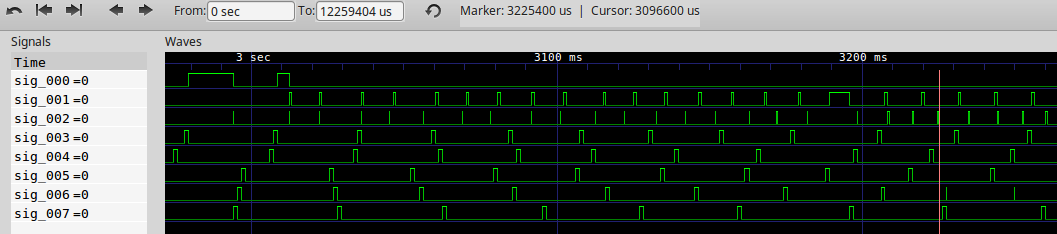
\includegraphics[scale=0.455]{../traces/traces1.png}
\captionof{figure}{Traces}
\end{center}
Pour rappel, l'ordre des tâches est le suivant : Game Task, Ball Task, Racket Task et les 5 Ghost Task.
À 3012 ms, le joueur a lancé le jeu, on aperçoit que la Game Task qui affichait le message "Press joystick"
s'arrête et laisse la place à la Ball Task. Le joystick est régulièrement vérifié dans la Racket Task et les
5 fantômes gardent un rythme régulier jusqu'à 3200 ms environ, à la position du curseur sur l'image. On voit
en effet qu'à 3189 ms, la Ball Task prend plus de temps, signe qu'il y a eu collision. On voit également que
le 4ème fantôme (pénultième tâche) prend moins de temps à s'exécuter à partir de 3227 ms, c'est lui qui a été
touché par la balle, il est devenu inactif. Les autres fantômes maintiennent leur durée d'exécution.
\newline
Nous voyons sur les traces que les durées des tâches sont maitrisées, il n'y a à aucun moment une ou plusieurs
tâches qui prennent la main pendant un temps trop long relativement aux autres, leur durée reste constante en
fonction du code exécuté.

\section{Limite du nombre de fantômes}
En augmentant le nombre de fantômes, nous pouvons observer un ralentissement du jeu.
Nous pouvons supposer que la fonction de récupération des traces n'est pas assez
performante et le buffer prend un certain temps pour se vider ce qui cause un ralentissement
général du jeu.
\newline
Nous avons remarqué aussi que le jeu reste bloqué lorsqu'il y a plus que 21 tâches
en parallèle. Nous pensons que cette limite vient de la mémoire allouée à FreeRTOS.
Au-delà de 21 tâches, on dépasse cette mémoire définie par la macro \mintinline{c}{configTOTAL_HEAP_SIZE}
définie ici à \mintinline{c}{20 * 1024}. En augmentant cette variable nous pouvons augmenter le
nombre de fantômes jusqu'à la limite de la mémoire de la carte. La limite que nous
avons atteint est de \mintinline{c}{configTOTAL_HEAP_SIZE = 27 * 1024} avec un nombre de tâches
de 29 (sans compter VApplicationIdleHook). Au-dessus nous avons un hardfault que
nous pensons être du à un dépassement de mémoire de la carte.

\section{Structure du programme}
\begin{center}
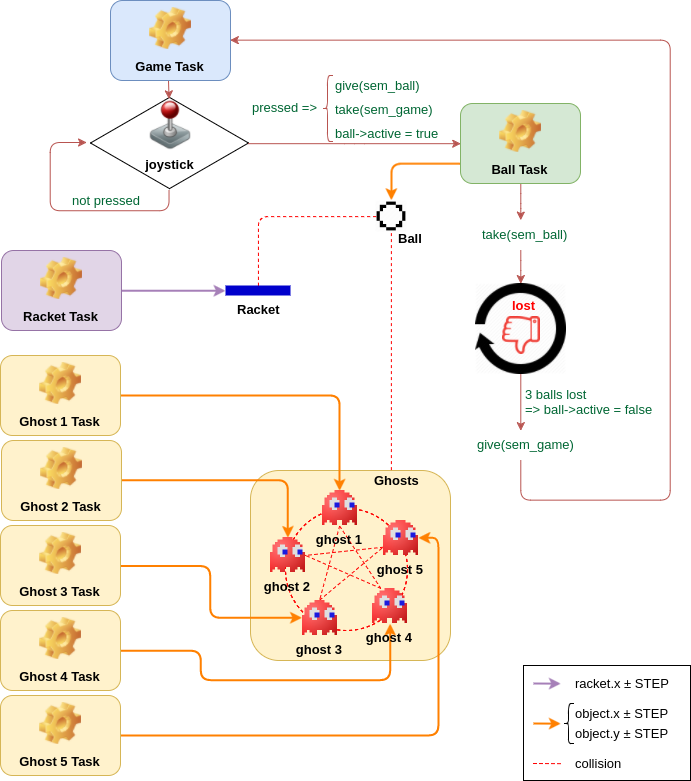
\includegraphics[scale=0.6]{ghostbusters.png}
\captionof{figure}{Schéma bloc du programme}
\end{center}

\end{document}
